%report.tex

%specify class of document
\documentclass[12pt, a4paper]{article}

%specify packages used 
\usepackage{microtype}		       %use package for minor typographical adjustments
\usepackage{graphicx} 		       %use package for diagram 
\usepackage{listings}                  %use package for c++ code in appendix
\usepackage{color}                     %use package for code listings
\usepackage[utf8]{inputenc}            %use package for colours in code
\usepackage{amsmath}                   %use package for various math symbols
\usepackage{amsfonts}                  %use package for number sets
\usepackage{bm}			       %use package for bolds in math mode
\usepackage{hyperref}                  %use package for hyperlinks
\usepackage{algpseudocode}             %use package for pseudocode
\usepackage{algorithm}                 %use package for pseudocode
\usepackage{fullpage}                  %use package for full page size
\usepackage{tikz}		       %use package for diagram drawings
\usepackage{caption}		       %use package for multiple figures
\usepackage{subcaption}                %use package for multiple figures
%\usepackage{url}                       %use package to display urls properly
%\usepackage{array}                     %use package for centering table contents

%set graphics path
\graphicspath{{/home/danmfr/p3t/laplace/images/}}

%define colours for code listings
\definecolor{codegreen}{rgb}{0,0.6,0}
\definecolor{codegray}{rgb}{0.5,0.5,0.5}
\definecolor{codepurple}{rgb}{0.58,0,0.82}
\definecolor{backcolour}{rgb}{0.95,0.95,0.92}

%define a style for the listings
\lstdefinestyle{mystyle}{
    backgroundcolor=\color{backcolour},
    commentstyle=\color{codegreen},
    keywordstyle=\color{magenta},
    numberstyle=\tiny\color{codegray},
    stringstyle=\color{codepurple},
    basicstyle=\footnotesize,
    breakatwhitespace=false,
    breaklines=true,
    captionpos=b,
    keepspaces=true,
    numbers=left,
    numbersep=5pt,
    showspaces=false,
    showstringspaces=false,
    showtabs=false,
    tabsize=2
}

%set style of listing to that defined above
\lstset{style=mystyle}

%use tikz library for shapes
\usetikzlibrary{shapes.geometric, arrows}

%define block styles in tikz
\tikzstyle{startstop} = [rectangle, rounded corners, minimum width=3cm, minimum height=1cm, text centered, draw=black, fill=red!30]
\tikzstyle{io} = [trapezium, trapezium left angle=70, trapezium right angle=110, minimum width=3cm, minimum height=1cm, text centered, draw=black, fill=blue!30]
\tikzstyle{process} = [rectangle, minimum width=3cm, minimum height=1cm, text centered, draw=black, fill=orange!30]
\tikzstyle{decision} = [diamond, minimum width=3cm, minimum height=1cm, text centered, draw=black, fill=green!30]
\tikzstyle{arrow} = [thick,->,>=stealth]

%set style of bibliography
\bibliographystyle{unsrt}

%set style of footnotes
\renewcommand{\thefootnote}{\roman{footnote}}

%define command shortcuts
\newcommand{\be}{\begin{equation}}
\newcommand{\ee}{\end{equation}}

%start of document
\begin{document}

%display title, my details and current date
\title{On numerical approximations to solutions of Laplace's equation for different electrostatic configurations}
\author{S. Brown, F. Hayes, L. Heikkil{\"a}, D. Richardson\\
	School of Physics and Astronomy,\\
	University of Glasgow,\\
	Glasgow, United Kingdom}
\date{\today}
\maketitle

%start of abstract
\begin{abstract}

The behaviour of the electric field under the presence and influence of solid
conducting objects is modelled and studied. Finite difference methods, namely
relaxation methods, are employed to solve the Laplace equation numerically,
to find the approximate form of the electrostatic potential, and hence the electric
field, present in various electrostatic systems.
We explicitly focus on two such systems: the case of a long perfectly conducting
cylinder centred between two infinite planes at potential $+V$ and $-V$; and the
case of a silicon detector---a system composed of two silicon wafers with segmented
doped implants at ground potential on one side and a uniform doped implant on the
other side, held at a potential $+V$. We compare the analytical solution of the first
system to its approximate numerical solution, and study the convergence of the
numerical methods employed.

\end{abstract} % end of abstract

%do not include in final version
\tableofcontents

%start of introduction
\section{Introduction}
\subsection{Laplace's Equation}

Gauss' Law may used to express the relation between the \emph{divergence} of the
electric field, represented by \textbf{E}, and the \emph{charge density} $\rho$,
where $\epsilon_0$ is the \emph{permittivity of free space}:
%
\be
\nabla \cdot \bm{E} = \frac{\rho}{\epsilon_0}
\ee
%
Alternatively (c.f. the Divergence Theorem), it can be expressed in its
integral form, as:
%
\be
\oint \limits_S \bm{E} \cdot d\bm{A} = \frac{Q}{\epsilon_0}
\ee
%
where the integral is taken over a closed surface, $S$, and $Q$ is the enclosed charge.
In the absence of charge, as is the case outside a conductor, this reduces to the
statement the electric field is \emph{solenoidal}.

One can also relate the \emph{curl} of the electric field to the time
derivative of the magnetic field, denoted \textbf{B}, by the Maxwell-Faraday equation:
%
\be
\nabla \times \bm{E} = - \frac{\partial \bm{B}}{\partial t}
\ee
%
If the magnetic field is constant, in other words unchanging with time, this equation
reduces to the statement that the electric field is \emph{irrotational}. A
consequence of irrotationality is that the electric field may then be written as
negative the gradient of some scalar potential, $\phi$ say. Mathematically:
%
\be
\bm{E} = -\nabla \phi
\ee
%
This scalar potential is called the \emph{electrostatic potential}.

One then has \emph{Laplace's equation}:
%
\be
\nabla^2 \phi = 0
\ee
%
where
$\nabla^2 \equiv \frac{\partial^2}{\partial x^2}+\frac{\partial^2}{\partial y^2}+\frac{\partial^2}{\partial z^2}$ 
is the \emph{Laplacian operator}\footnote{Specifically in Cartesian co-ordinates}.

This is a second-order partial differential equation that can be solved, given some
well-posed boundary conditions, to find the electrostatic potential and electric field
for some physical system. 

This equation is found in many areas of physics, from studies of fluid dynamics and heat
conduction to astronomy, and our analysis here could be generalised to other such areas
of physics.

\subsection{Finite Difference Methods}

It is often the case that differential equations, such as the Laplace equation, cannot
be solved analytically, and their solution must be numerically approximated.

To numerically approximate the solution to a differential equation it is
necessary to approximate the derivative of a function. The usual method employed to
do this is finite differencing. This approximates the derivative by using explicit
differencing to step the function from one value to the next in small 
increments of some variable. The smaller the increment used, the more accurate
the approximation, but the longer and more computationally intensive the process.

Suppose one wishes to approximate the first derivative of a function $f(t)$, say,
with respect to the variable $t$. The simplest way to do this is to discretise the
derivative and write
%
\be
\frac{df}{dt} \approx \frac{f(t+\Delta t) - f(t)}{\Delta t}
\ee
%
where $f(t+\Delta t)$ and $f(t)$ are two values of $f$, evaluated at two points
a distance $\Delta t$ apart. This is known as the \emph{forward difference approximation}.

To approximate the second derivative of a function, one writes
%
\be
\frac{d^2 f}{dt^2} \approx \frac{f'(t) - f'(t-h)}{\Delta t} \\
= \frac{\frac{f(t +\Delta t) - f(t)}{\Delta t} - \frac{f(t) - f(t -\Delta t)}{\Delta t}}{\Delta t} \\
= \frac{f(t +\Delta t) - 2f(t) + f(t-\Delta t)}{\Delta t ^2}
\ee

\subsection{System Desricption}
\subsubsection{System One}

Suppose one has a perfectly uniform electric field between two infinite planes
at potentials $V$ and $-V$, and they are a distance $2d$ apart. Suppose one then
places an infinitely long perfectly conducting cylinder, of radius $R$, into the centre
of the field, at ground potential, as in Figure~\ref{fig:sys one}. We wish to find the
resulting form of the electrostatic potential, and hence the electric field, surrounding
the cylinder.

\begin{figure}[h!]
\begin{center}
\begin{tikzpicture}
\draw (0,0) node[below] {$x = -d$} -- (0,6) node[above] {$\phi = V$}; 
\draw (10,0) node[below] {$x = d$} -- (10,6) node[above] {$\phi = -V$}; 
\draw (5,3) circle (1cm) node[below] {$\phi=0$};
\draw[dashed] (5,3) -- (5.6,3.8) node[pos=0.5,above left] {$R$};
\end{tikzpicture}
\end{center}
\caption{Cross-sectional diagram of System One}
\label{fig:sys one}
\end{figure}

\subsubsection{System Two}

The second system considered was a silicon detector---a system consisting of two
silicon wafers, one segmented with doped implants at ground potential and the other,
referred to as the backplane, uniformly doped, held at a potential $+V$, as shown
in Figure~\ref{fig:sys two}.

\begin{figure}[h!]
\begin{center}
\begin{tikzpicture}
\draw (0,0) -- (12,0) node[right] {$\phi = V$}; 
\draw (0,5) -- (12,5) node[pos=0.25, above] {GND} node[pos=0.5, above] {GND} node[pos=0.75,above] {GND}; 
\draw (2.5,5) rectangle (3.5,4.75);
\draw (5.5,5) rectangle (6.5,4.75);
\draw (8.5,5) rectangle (9.5,4.75);
\end{tikzpicture}
\end{center}
\caption{Cross-sectional diagram of System Two}
\label{fig:sys two}
\end{figure}

\subsection{Analytical Solution to System One}

First, one realises that the three-dimensional problem can be reduced entirely to two
dimensions due to the translation symmetry of the system along the length of the
cylinder. So, we consider a cross-section of the system and introduce a polar
co-ordinate system, with origin centred on the centre of the cylinder.

Laplace's equation in polar co-ordinates is: 
%
\be
\frac{\partial^2 \phi}{\partial r^2}+\frac{1}{r}\frac{\partial \phi}{\partial r}+\frac{1}{r^2}\frac{\partial^2 \phi}{\partial \theta^2}
= \frac{1}{r}\frac{\partial}{\partial r}(r \frac{\partial \phi}{\partial r}) + \frac{1}{r^2}\frac{\partial ^2 \phi}{\partial \theta^2}
= 0
\ee

We employ separation of variables and posit a solution of the form
$\phi = f(r)g(\theta)$ for two unknown functions $f$ and $g$. Upon substitution,
one finds that:
%
\be
\frac{r}{f(r)}\frac{d}{dr}(r \frac{df(r)}{dr}) =- \frac{1}{g(\theta)}\frac{d^2 g(\theta)}{d\theta^2}
\ee

Since this is true for arbitrary values of $r$ and $\theta$, it is constant, and
we---with some foreknowledge---set this equal to $k^2$, for some constant 
$k\in\mathbb{R}$.
This gives two second order ordinary differential equations:
%
\be
r\frac{d}{dr}(r \frac{df(r)}{dr}) = k^2 f(r) \qquad
\frac{d^2 g(\theta)}{d\theta^2}=-k^2 g(\theta)
\ee

For the case $k=0$, these equations have solutions
$f(r)=\alpha \ln(r) + \beta$ and $g(\theta) = \gamma \theta + \delta$.
For non-zero $k$, they have solutions
%
\be
f(r)=\alpha_k r^k + \beta_k r^{-k}
\qquad
g(\theta)= \gamma_k \sin(k\theta)+\delta_k \cos(k\theta)
\ee

With the physically reasonable requirement that $g(\theta)=g(\theta + 2\pi)$, we have
that $k$ is an integer. Hence, by the principle of superposition and the linearity of
differentiation, the general solution to the Laplace equation in polar co-ordinates is
a sum of these terms:
%
\be
\phi(r,\theta)
= f(r)g(\theta)
= (\alpha \ln(r) + \beta)(\gamma\theta + \delta) + \sum_{n=1}^{\infty}(\alpha_n r^n+\beta_n r^{-n})(\gamma_n \sin(n\theta) + \delta_n \cos(n\theta))
\ee

For a particular solution to the system considered here one must impose boundary
conditions, specifically we use \emph{Dirichlet boundary conditions}.

By considering the geometry of the system, we expect a solution that is symmetric
about $\theta=0$. This implies that $\gamma = 0$ and $\gamma_n=0$, $\forall n$ as
$\sin()$ is anti-symmetric about the origin (c.f. odd). Additionally, the potential
is finite as $r \rightarrow \infty$, implying that $\alpha$ and $\alpha_n$ are both
zero. We now have:
%
\be
\phi(r,\theta)=\beta + \sum_{n=1}^{\infty}(\frac{\beta_n}{r^n} \cos(n\theta))
\ee
%
where the $\beta$'s have absorbed other constants. In particular, as
$r \rightarrow \infty$, we require $\phi=-\frac{V}{d}x=-\frac{V}{d}r\cos(\theta)$.
Since the infinite sum vanishes at infinity, $\beta=-\frac{V}{d}r\cos(\theta)$.

We now have that
%
\be
\phi(r,\theta)=-\frac{V}{d}r\cos(\theta) + \sum_{n=1}^{\infty}(\frac{\beta_n}{r^n} \cos(n\theta))
              =(\frac{\beta_1}{r}-\frac{V}{d}r)\cos(\theta) + \sum_{n=2}^{\infty}(\frac{\beta_n}{r^n} \cos(n\theta))
\ee

We require that the potential is zero on the surface of the cylinder,
$\phi(R,\theta)=0$, so that $\beta_1=\frac{VR^2}{d}$ and $\beta_{n \geq 2}=0$

Thus, the final form for the electrostatic potential is
%
\be
\phi(x,y)=
\begin{cases} \qquad 0, & \quad r \leq a \\
\frac{V}{d}(\frac{R^2}{r}-r)\cos(\theta), & \quad r > a
\end{cases}
\ee
%
a graph of which is shown in Figure~\ref{fig:analytic}.

\begin{figure}
\begin{center}
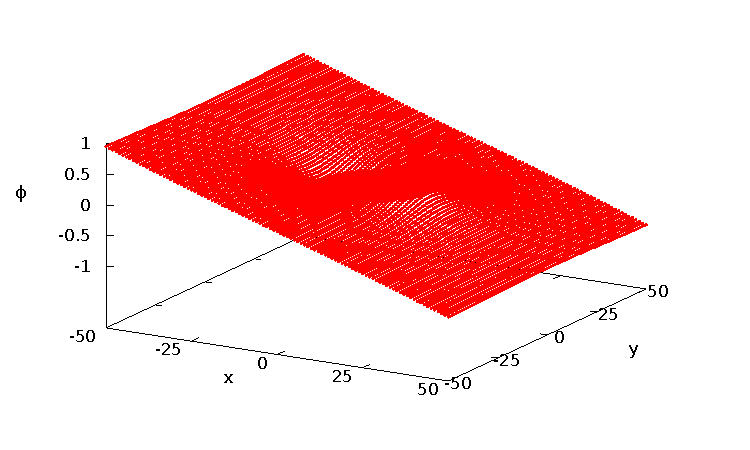
\includegraphics{analytic.pdf}
\caption{Analytic solution with $V=1$, $R=15$ on $100\times100$ grid}
\label{fig:analytic}
\end{center}
\end{figure}

\section{Relaxation Methods}

\subsection{Jacobi's Iterative Method}

For our purposes, we wish to discretise the following equation:
% 
\be 
\frac{\partial^2 \phi}{\partial x^2}+\frac{\partial^2 \phi}{\partial y^2} = 0
\label{eq:laplace}
\ee 

One can define a region on which to discretise this equation, $\{(x,y)|\:0<x<L,0<y<D\}$,
and define a grid of points of spacial separation in $\Delta x$ in the $x$ direction,
and $\Delta y$ in the $y$ direction. We wish to find the value of $\phi$ at each point.

One can now approximate Eqn.~\ref{eq:laplace} as:
% 
\be
\frac{\phi_{j+1,k}-2\phi_{j,k}+\phi_{j-1,k}}{\Delta x^2} = - \frac{\phi_{j,k+1}-2\phi_{j,k}+\phi_{j,k-1}}{\Delta y^2}
\ee
%
where $j$ and $k$ index the $x$ and $y$ directions respectively.

If we use the same spacing $\Delta=\Delta x=\Delta y$ in both $x$ and $y$ directions this
reduces to the statement that the value of the potential at a specific point is the
average of the value of the potential at the four surrounding points: 
%
\be
\phi_{j,k}= \frac{1}{4}(\phi_{j-1,k}+\phi_{j+1,k}+\phi_{j,k-1}+\phi_{j,k+1})
\label{eq:relax}
\ee

Suppose one has some initial guess of the value of $\phi$ at all points, $\phi_{j,k,0}$,
say. One evaluates Eqn~\ref{eq:relax} at all points on the grid simultaneously and
generates a new better approximation for the potential, $\phi_{j,k,1}$. Iterating this
process $n$ times, one has
%
\be
\phi_{j,k,n+1}= \frac{1}{4}(\phi_{j-1,k,n}+\phi_{j+1,k,n}+\phi_{j,k-1,n}+\phi_{j,k+1,n})
\ee
%
This is known as \emph{Jacobi's iterative method}, the simplest version of a
\emph{relaxation method}, an algorithm where the numerical approximation converges or
\emph{relaxes} towards the analytical solution with increasing iterations. 

\subsection{The Gauss-Seidel Method}

An alternative relaxation method, known as the \emph{Gauss-Seidel method}, exists where
points at which the potential has already been updated by the algorithm as it loops
through the grid, namely $\phi_{j-1,k}$ and $\phi_{j,k-1}$ in our notation, are used in
the iteration scheme, as shown:
%
\be
\phi_{j,k,n+1}= \frac{1}{4}(\phi_{j-1,k,n+1}+\phi_{j+1,k,n}+\phi_{j,k-1,n+1}+\phi_{j,k+1,n})
\ee

It can be shown that this method actually converges faster than Jacobi's iterative
method, and it also has the added bonus of not requiring the previous value of the 
potential at each grid point to be stored, thus reducing computation time.

\subsection{Successive Over-Relaxation}

Neither the Jacobi iterative method or the Gauss-Seidel method utilise the value
of the potential at the current point in the previous iteration, in our notation
$\phi_{j,k,n}$. It can be shown that using this point, and defining a
\emph{relaxation parameter}, $1<s<2$, one can define the following iterative algorithm:
%
\be
\phi_{j,k,n+1}= (1-s)\phi_{j,k,n}+\frac{s}{4}(\phi_{j-1,k,n+1}+\phi_{j+1,k,n}+\phi_{j,k-1,n+1}+\phi_{j,k+1,n})
\ee
%
which is a more convergent numerical method. This technique is known as successive
over-relaxation.

%add fergus
%input{sor.tex}

\subsection{Checkerboard (Red-Black) Updating}

In each of the previous methods, the value of the potential is calculated from, at most,
its previous value at the current point and the current or previous values of the
potential at the four neighbouring points. Noting this, let us denote $\phi_{j,k}$ as
\emph{odd} if $j+k$ is odd, and even otherwise. Then the potential at each even point
solely depends on the potential at odd points (and its previous value). One could then,
in principle, iterate through the grid of points at which we approximate the potential,
and update all the odd points, and then re-iterate through the grid, updating all the
even points using the value of the potential at the newly updated odd points. Such an
iterative scheme exists, and is known as Checkerboard (Red-Black) Updating, for obvious
reasons. It can be shown to be a more convergent method than those outlined previously,
and successive over-relaxation can easily be implemented within the scheme.

%add stephen
%\input{checker.tex}

%add fergus
\subsection{Nine-point Stenciling}
%The previous expression for the Laplace equation to find the potential of point $(x,y)$
using points $(x,y+h)$, $(x,y-h)$, $(x-h,y)$ and $(x+h,y)$ can be expanded to
include the points $(x+h,y+h)$, $(x+h,y-h)$, $(x-h,y+h)$ and $(x-h,y-h)$. This is
done by incorporating the Taylor expansion for the new points with the
previous expression. The Laplace equation becomes:
%
\begin{align}
\nabla ^2 \phi &= \frac{4(\phi_{i+1,j} + \phi_{i-1,j} + \phi_{i,j-1} + \phi_{i,j+1})}{6h^2} \nonumber \\
&+ \frac{\phi_{i+1,j-1} + \phi_{i+1,j+1} + \phi_{i-1,j-1} + \phi_{i-1,j+1}}{6h^2} \nonumber \\
&- \frac{20\phi_{i,j}}{6h^2} - \frac{h^2(\phi_{xxxx} + 2 \phi_{xxyy} + \phi_{yyyy})}{6} - O(h^4)
\end{align}

The truncation error associated with the expression is second order. However, the terms
inside the bracket $(\phi_{xxxx} + 2 \phi_{xxyy} + \phi_{yyyy})$ is equal to the
Laplacian of the Laplacian of the potential $\nabla^2 (\nabla ^2 \phi)$. For the case
for the Laplace equation, $\nabla ^2 \phi = 0$ and therefore the second order term in
the expression is reduced to zero and the truncation error becomes fourth order. This
allows the nine-point stencil to be more accurate with less iterations than the
five-point stencil. However, the larger calculations have a computational cost and
increases the time spent on each iteration.


\subsection{Comparison of methods}

This is the scheme we shall use to numerically approximate the electrostatic potential
in different . 

%start of section
%section is still under work, and out of order
\section{Software Package for general electrostatic systems, \emph{estatics}}

To numerically approximate the electrostatic potential for System 1 via the 
relaxation method the following rudimentary algorithm was developed.

\begin{algorithm}
\begin{algorithmic}[1]
\Procedure{The Relaxation Method}{}
\State declare variables:
\State $V \gets$ potential on plates
\State $\delta \gets$ position step-size
\State $d \gets$ distance between plates
\State $h \gets$ height of plates
\State $r \gets$ radius of cylinder
\State $its \gets$ number of iterations
\State $nx \gets \frac{d}{\delta}$ 
\State $ny \gets \frac{h}{\delta}$ 
\State specify boundary potentials:
\For {$j=1$ to $ny$}
   \State $u_{j, 1} = +V$
   \State $u_{j, nx} = -V$
\EndFor
\For {$k=1$ to $nx$}
   \State $u_{1, k} \gets V-\frac{2Vj}{nx}$
   \State $u_{ny, k} \gets V-\frac{2Vj}{nx}$
\EndFor
\State find solution:
\For {$i=1$ to $its$}
   \For {$j=2$ to $ny-1$}
      \For {$k=2$ to $nx-1$}
         \If {$(j \delta-\frac{1}{2} d)^2+(k \delta-\frac{1}{2} h)^2<r^2$}
            \State $u_{j, k} \gets 0$
         \Else
            \State $u_{j,k} \gets \frac{1}{4}(u_{j-1,k}+u_{j+1,k}+u_{j,k-1}+u_{j,k+1})$
         \EndIf
      \EndFor
   \EndFor
\EndFor
\State find electric field:
\For {$j=1$ to $ny-1$}
   \For {$k=1$ to $nx-1$}
      \State $(Ex)_{j, k} \gets -\left(u_{j,k+1}-u_{j,k}\right)/\delta$
      \State $(Ey)_{j,k} \gets -\left(u_{j+1,1}-u_{j,k}\right)/\delta$
   \EndFor
\EndFor
\State plot potential and field
\EndProcedure
\end{algorithmic}
\end{algorithm}

Figure~\ref{fig:numerical} shows the numerical approximation to the potential,
and Figure~\ref{fig:field} shows the electric field around the cylinder.

\begin{figure}
\centering
\begin{subfigure}[b]{0.7\textwidth}
	\includegraphics[width=\textwidth]{potentialA.pdf}
	\caption{electrostatic potential}
	\label{fig:numerical}
\end{subfigure}

\begin{subfigure}[b]{0.7\textwidth}
	\includegraphics[width=\textwidth]{fieldA.pdf}
	\caption{electric field}
	\label{fig:field}
\end{subfigure}
\caption{Numerical approximations for electstatic potential and electric field with
$V=1$, $R=15$ on $100\times100$ grid for $10000$ iterations}
\end{figure}

We developed a general software package in C++ to solve and plot the potential and
electric field for an arbitrary electrostatic system. It accepts input of a coloured
bitmap, where the colours represent different potentials, and returns plots of the
resultant electrostatic potential and electric field.

Figure~\ref{fig:flowchart} shows a flowchart representing the algorithm employed.

\begin{figure}[htbp!]
\begin{center}
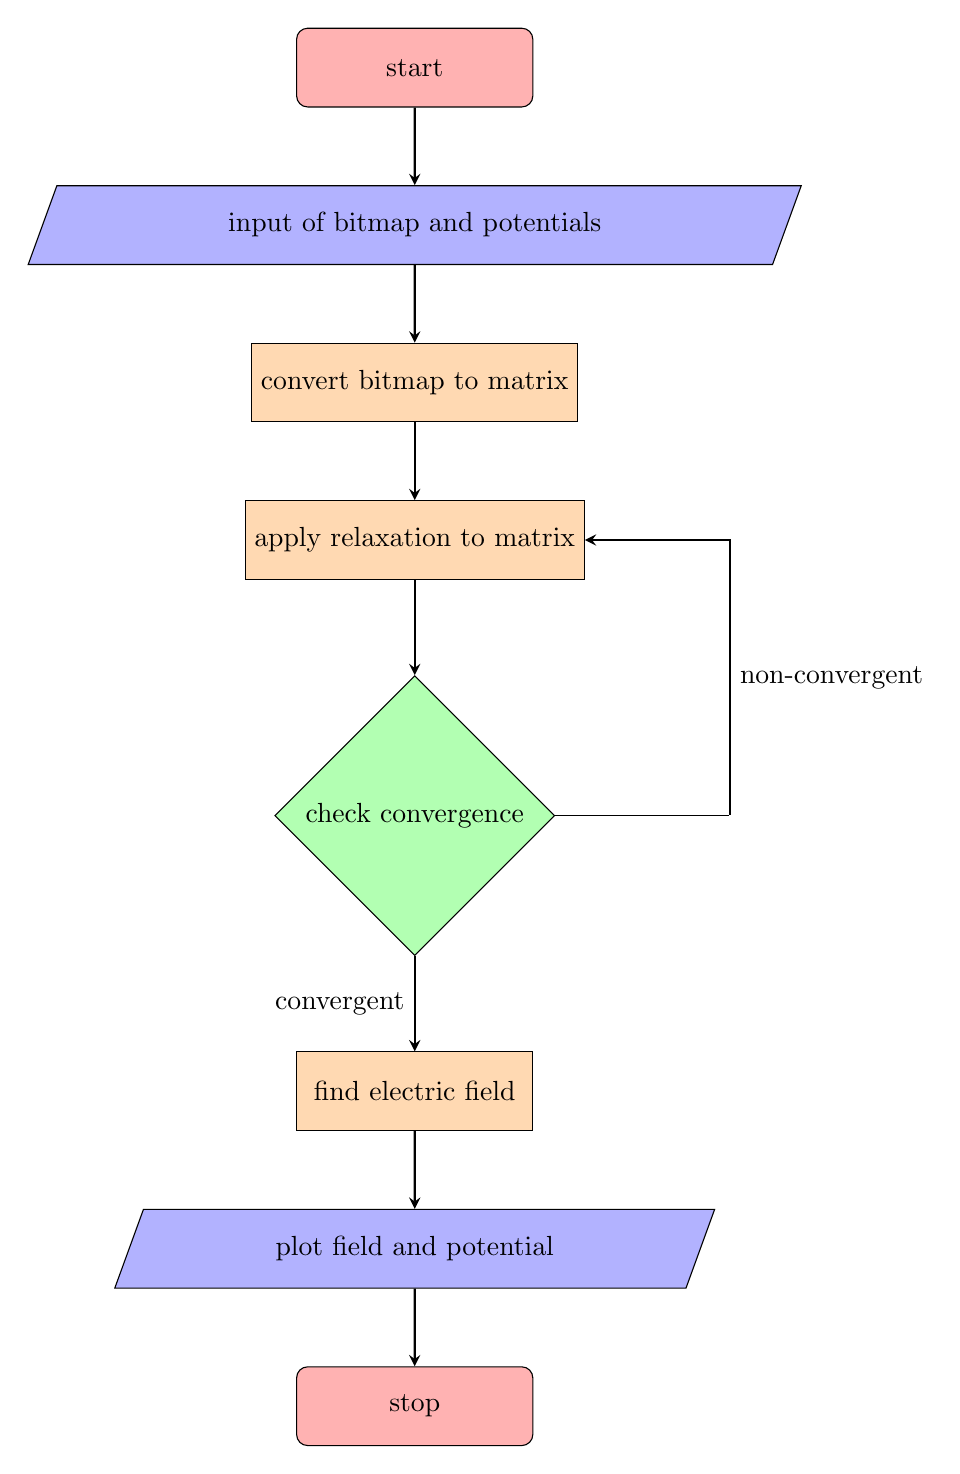
\begin{tikzpicture}[node distance=2cm]

\node (start) [startstop] {start};
\node (in1) [io, below of=start] {input of bitmap and potentials};
\node (pro1) [process, below of=in1] {convert bitmap to matrix};
\node (pro2) [process, below of=pro1] {apply relaxation to matrix};
\node (dec1) [decision, below of=pro2, yshift=-1.5cm] {check convergence};
\node (inv) [inner sep=0, minimum size=0, right of=dec1, xshift=2cm] {}; % invisible node
\node (pro3) [process, below of=dec1, yshift=-1.5cm] {find electric field};
\node (out1) [io, below of=pro3] {plot field and potential};
\node (stop) [startstop, below of=out1] {stop};

\draw [arrow] (start) -- (in1);
\draw [arrow] (in1) -- (pro1);
\draw [arrow] (pro1) -- (pro2);
\draw [arrow] (pro2) -- (dec1);
\draw [arrow] (dec1) -- node[left] {convergent} (pro3);
\draw (dec1) -- (inv);
\draw [arrow] (inv) |- node[pos=0.25, right] {non-convergent} (pro2);
\draw [arrow] (pro3) -- (out1);
\draw [arrow] (out1) -- (stop);

\end{tikzpicture}
\end{center}
\caption{Flowchart of steps in software package}
\label{fig:flowchart}
\end{figure}

%adds fergus' section
\subsection{Bitmaps}
%Unlike PNG, GIF and JPEG image files, BMP files are uncompressed allowing them to be manipulated easily by programs. In a BMP file, there are three bytes of memory for each pixel to store a value for the colour scale for three different colours: blue, green and red. The colour scale runs from 0 to 255 (0 being no contribution from that colour to the pixels colour and 255 being maximum contribution) and allows the pixel to have a range of 16,777,216 individual variations in colour.

The potential boundaries for each system were drawn onto a blank BMP file where coloured areas are areas of constant potential and blank white pixels are areas of unsolved potential. Each colour has a different value of potential to assign to the points it covers. For the systems examined, only a minimum of four different potentials were needed and therefore were represented by the colours black, red, green and blue. The potential assigned to each colour was taken off the command line arguments. The strengths of green, blue and red can be determined comparing which colour scale is largest, and black is simply the absence of any values for the colour scales (BMP files of both the systems are found in the Appendix~\ref{app:bitmaps}).

eStatics analyses each pixels colour and maps boundary conditions onto arrays of the same dimensions as the pixel array, these arrays are: the potential grid stores the potential of the boundaries and the unsolved areas (initially set to zero) and the bool mask which stores boolean elements set to true at boundary locations and false at unsolved areas to keep boundaries constant. To extract the information from the BMP files, a library of commands called 'bitmap\textunderscore image.hpp'~\cite{arash} was used. This allowed the program to open the BMP file  by taking the file name from a command line argument before extracting the dimensions of the image and assigning the width and height to integers.

The pixel array is looped through and integers are assigned with the value of the colour scale. The colour of the pixel is determined by comparing the colour scales; if the red colour scale is greater than the blue and green colour scales, then the point on the potential grid is given the potential from the command line arguments assigned to red pixels and \emph{vice-versa} for green and blue. If the colour scales all equal zero, then the colour of the pixel is said to be black. The value on the potential grid with the same location as the pixel is assigned with the value of potential associated with the pixels colour. Points on the boolean array at the locations of coloured pixels is set to true.


%fergus
\subsection{Convergence}
%The successive over-relaxation method does not have an easily quantifiable error. The truncation error from the finite difference approximation is found by calculating higher derivatives than the solution requires and therefore requires substantially more computing to determine. Instead the precision of our results are analysed.
\\
The precision is related to how close a numerically determined value is from the true value it is converging to. If a numerical process determines a value $\tilde{x}$ on iteration $n$ which is converging to $x$, then:
\begin{align*}
\lim_{n \rightarrow \infty}\tilde{x} = x                     
\end{align*}
As the true value $x$ is constant, if the expression is differentiated with respect to the number of iterations, the rate of change of the determined value $\tilde{x}$ over iterations tends towards zero:
\begin{align*}
\lim_{n \rightarrow \infty}\frac{d\tilde{x}}{dn} = \lim_{n \rightarrow \infty} (\tilde{x}^{n} - \tilde{x}^{n-1}) = 0                     
\end{align*}
The magnitude of the difference of determined values $\tilde{x}$ between successive iterations is then related to how close the value is to the true value $x$. The closer the value is to zero, the more precise the value.
\subsection{Absolute Convergence}
The magnitude of the difference of the potential between successive iterations at some point is referred to as absolute convergence $\epsilon_{abs}$ of that point:
\begin{align*}
\epsilon_{abs \; i,j}^{n} = |\tilde{\phi}^{n} - \tilde{\phi}^{n-1}|
\end{align*}
This value is used in the program to limit the number of iterations the numerical process undertakes and also is used to 'lock' converged points to reduce calculations per iteration.
\subsection{Convergence Limit}
Within the program, the precision of the numerical solution is analysed as an indicator of accuracy. The absolute convergence is found for every point on the potential grid to determine the convergence of the system.
\\
The number of iterations the program carries out for a system can be made dependent on the convergence; the system can be iterated over until all the points meet a desired absolute convergence $\epsilon$. This desired absolute convergence is taken from the command line arguments and is a value typically between $10^{-3}$ and $10^{-12}$. When every points absolute convergence has fallen below the desired absolute convergence, $\epsilon_{abs} < \epsilon$, the system is said to be converged. 
\\
The successive over-relaxation method iterates within a while loop. This while loop is conditioned so that it loops through the potential grid with the successive over-relaxation method until the 'convergence count' is equal to the number of points on the grid (number of pixels of the image). The convergence count is set to zero at the start of each iteration, and it is incremented by one for every point that has a absolute convergence less than the desired absolute convergence.


%stephen
\subsection{Data Handling}
%		In order to simplify the passing of pertinent data to and from sub-functions, two structs were created. Structs --- or records --- are a type of data structure which can hold an arbitrary number of fields, each of which can be of a different data type. This makes them ideal for this case; arrays of type \lstinline|double| are required to hold the system to be solved and the gradient components of the electric field, \lstinline|int| variables can be used to hold the dimensions of the array --- which allows the solver to simply read this information rather than calculate it when needed - and to pass back the number of iterations required to meet the desired convergence, and the \lstinline|bool| data type can be used to write-protect boundary elements. This final point is discussed in detail in section~\ref{sec:mask}.
		
		In the case of \lstinline|eStatics|, a global pointer to the data struct was defined as \lstinline|extern| in the header file and created outside the main function. This allows the designation of a memory address to the structure which can be seen by all sub-routines, allowing each to read from and write to the fields contained within it. The \lstinline|new| command is used to dynamically assign memory to those fields, and expand them when needed. This allows systems of arbitrary size, or fineness of grid, to be solved by the software package. Another benefit of using a global struct is that variables such as system dimension, desired convergence, and maximum iterations need only be written once when building the system --- from then on only memory reads are required. Finally, RAM usage is lowered due the passing of only one set of data by address; this is due to there being no need to copy data and pass it by value to sub-routines.

%adds stephen's section, uncomment and compile
\subsection{Boolean Masks and Locking}
%		A problem with iterative algorithms such as the Finite Difference Method (FDM) is that the initial boundary conditions can be eroded by successive averaging. To counteract this, these boundaries must either be rewritten with each iteration --- with significant costs in terms of time due to extra read/write cycles being required, and RAM usage due to a copy of the initial grid having to be kept in memory --- or write-protected for the duration of the program. For the latter, which can avoid or reduce the noted costs of the former, the boolean data type is ideally suited.
		
		\subsubsection{Boolean Mask}
		
		Boolean is a data type with only two possible values; true or false. As such, each boolean --- or \lstinline|bool| --- requires very little memory. Typically, a boolean variable is the smallest possible variable in terms of RAM requirements. This makes them ideal for use in the write-protection of boundary elements, as it drastically lowers the overhead in this area. In order to utilise this, a boolean array of equal dimension to the system array is created whilst the user-provided bitmap image is being analysed. If an element, or pixel, of the system is defined as a boundary element the corresponding element in the boolean mask is set to true. All non-boundary elements are set to false.
		
		Next, whilst the solver is running through the system array point-by-point, it first checks the corresponding element in the mask. If this boolean is found to be true, the solver ignores that element. This saves time, as no further calculation needs to take place on that element.


\subsection{Timing and CPU usage}

%adds lassi's section, uncomment and compile
\subsection{Output and Plotting}
%% plotting.tex - to be inserted into the the main report.tex file


%specify class of document
\documentclass[12pt, a4paper]{article}

%specify packages used 
\usepackage{microtype}           %use package for minor typographical adjustments
\usepackage{graphicx}            %use package for diagram 
\usepackage{listings}                  %use package for c++ code in appendix
\usepackage{color}                     %use package for code listings
\usepackage[utf8]{inputenc}            %use package for colours in code
\usepackage{amsmath}                   %use package for various math symbols
\usepackage{amsfonts}                  %use package for number sets
\usepackage{bm}            %use package for bolds in math mode
% \usepackage{hyperref}                  %use package for hyperlinks
% \usepackage{algpseudocode}             %use package for pseudocode
% \usepackage{algorithm}                 %use package for pseudocode
% \usepackage{fullpage}                  %use package for full page size
% \usepackage{tikz}          %use package for diagram drawings
% \usepackage{caption}           %use package for multiple figures
% \usepackage{subcaption}                %use package for multiple figures
%\usepackage{url}                       %use package to display urls properly
%\usepackage{array}                     %use package for centering table contents
\usepackage[scale=0.80]{geometry}
\usepackage{tabularx}

%start of document
\begin{document}


\section{Outputting and plotting the results} % explain what the output files look like and how they are plotted
The final matrix contains the numerical value of the electric potential at each point in the grid as a number of type \emph{double}. The program outputs the value of each point along the y-direction corresponding to an x-value, then moves on to the next x-value and repeats the process. The program writes the value of the potential at each point to a file in the format shown in table \ref{table:potential_data}.

After all y values have been outputted for an x value, the final row is followed by an empty row before the next x value is started. This is done to allow gnuplot to plot three dimensional data. This file is used to plot the potential as a heatmap-styled plot, an example of which can be seen in figure \ref{fig:potentialplot}.

\begin{figure}[h!]
\centering
\setlength\fboxsep{0pt}
\setlength\fboxrule{0.5pt}
\fbox{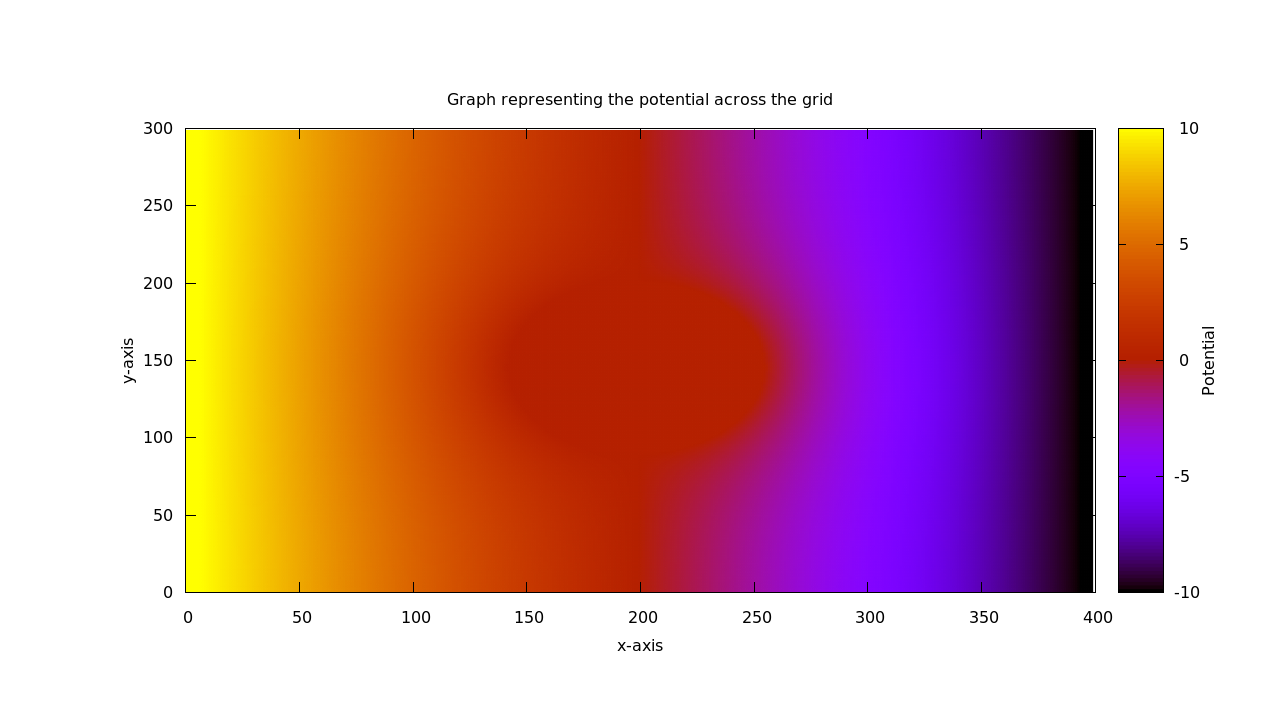
\includegraphics[width=0.95\textwidth, trim = 40mm 20mm 20mm 30mm, clip]{example_potential_plot.png}} % change trim as required to eliminate unnecessary whitespace. trim: left bottom right top
\label{fig:potentialplot}
\caption{A plot representing the electric potential ${\phi}$ at points in the grid.}
\end{figure}

Another output file is also produced to allow the plotting of the electric field. The file contains the x- and y-coordinates as well as the $d{\phi}/dx$ and $d{\phi}/dy$ values, which are approximated. For a point $(x,y)$, the gradient along the x-direction is calculated as the average of the change along one step from the left (-x direction) and one step to the right (+x direction), i.e. $d{\phi}/dx_{x,y} = ( value(x-1,y) - value(x+1,y) ) / 2$. Similarly, for the gradient along the y-direction, the gradient is calculated as the average of the change along one step to the +y direction and one step from the -y direction, i.e. $d{\phi}/dy_{x,y} = ( value(x,y-1) - value(x,y+1) ) / 2$. Here the $\phi$ refers to the potential. The values are written to a file in the format shown in table \ref{table:field_data}.
\begin{table}
    \parbox{0.47\linewidth}{
    \centering
    \begin{tabularx}{0.44\textwidth}{ |XXX| }
        \hline
        $x_1$ & $y_1$ & $value_{1,1}$ \\
        $x_1$ & $y_2$ & $value_{1,2}$ \\
        $x_1$ & $y_3$ & $value_{1,3}$ \\
        & & \\
        $x_2$ & $y_1$ & $value_{2,1}$ \\
        $x_2$ & $y_2$ & $value_{2,2}$ \\
        $x_2$ & $y_3$ & $value_{2,3}$ \\
        & & \\
        $x_3$ & $y_1$ & $value_{3,1}$ \\
        $x_3$ & $y_2$ & $value_{3,2}$ \\
        $x_3$ & $y_3$ & $value_{3,3}$ \\
        \hline
    \end{tabularx}
    \caption{Structure of a file containing information about the potential across the grid. This example is for a 3x3 grid.}
    \label{table:potential_data}
    }
    \hfill
    \parbox{0.47\linewidth}{
    \centering
    \begin{tabularx}{0.44\textwidth}{ |XXXX| }
        \hline
        $x_1$ & $y_1$ & $d{\phi}/dx_{1,1}$ & $d{\phi}/dy_{1,1}$ \\
        $x_1$ & $y_2$ & $d{\phi}/dx_{1,2}$ & $d{\phi}/dy_{1,2}$ \\
        $x_1$ & $y_3$ & $d{\phi}/dx_{1,3}$ & $d{\phi}/dy_{1,3}$ \\
        & & & \\
        $x_2$ & $y_1$ & $d{\phi}/dx_{2,1}$ & $d{\phi}/dy_{2,1}$ \\
        $x_2$ & $y_2$ & $d{\phi}/dx_{2,2}$ & $d{\phi}/dy_{2,2}$ \\
        $x_2$ & $y_3$ & $d{\phi}/dx_{2,3}$ & $d{\phi}/dy_{2,3}$ \\
        & & & \\
        $x_3$ & $y_1$ & $d{\phi}/dx_{3,1}$ & $d{\phi}/dy_{3,1}$ \\
        $x_3$ & $y_2$ & $d{\phi}/dx_{3,2}$ & $d{\phi}/dy_{3,2}$ \\
        $x_3$ & $y_3$ & $d{\phi}/dx_{3,3}$ & $d{\phi}/dy_{3,3}$ \\
        \hline
    \end{tabularx}
    \label{table:field_data}
    \caption{Structure of a file containing information about the electric field across the grid. This example is for a 3x3 grid.}
    }
\end{table}

Again, empty lines are inserted before a change in x-values to make operating gnuplot easier. The data can then be plotted as a vector field in, for example, gnuplot. By setting some functions in gnuplot, one can make the vectors in the field of uniform size (to improve readability) and indicate the magnitude of the vector by colour. An example of such a plot can be seen in figure \ref{fig:vectorfieldplot}.

\begin{figure}[h!]
    \centering
    \setlength\fboxsep{0pt}
    \setlength\fboxrule{0.5pt}
    \fbox{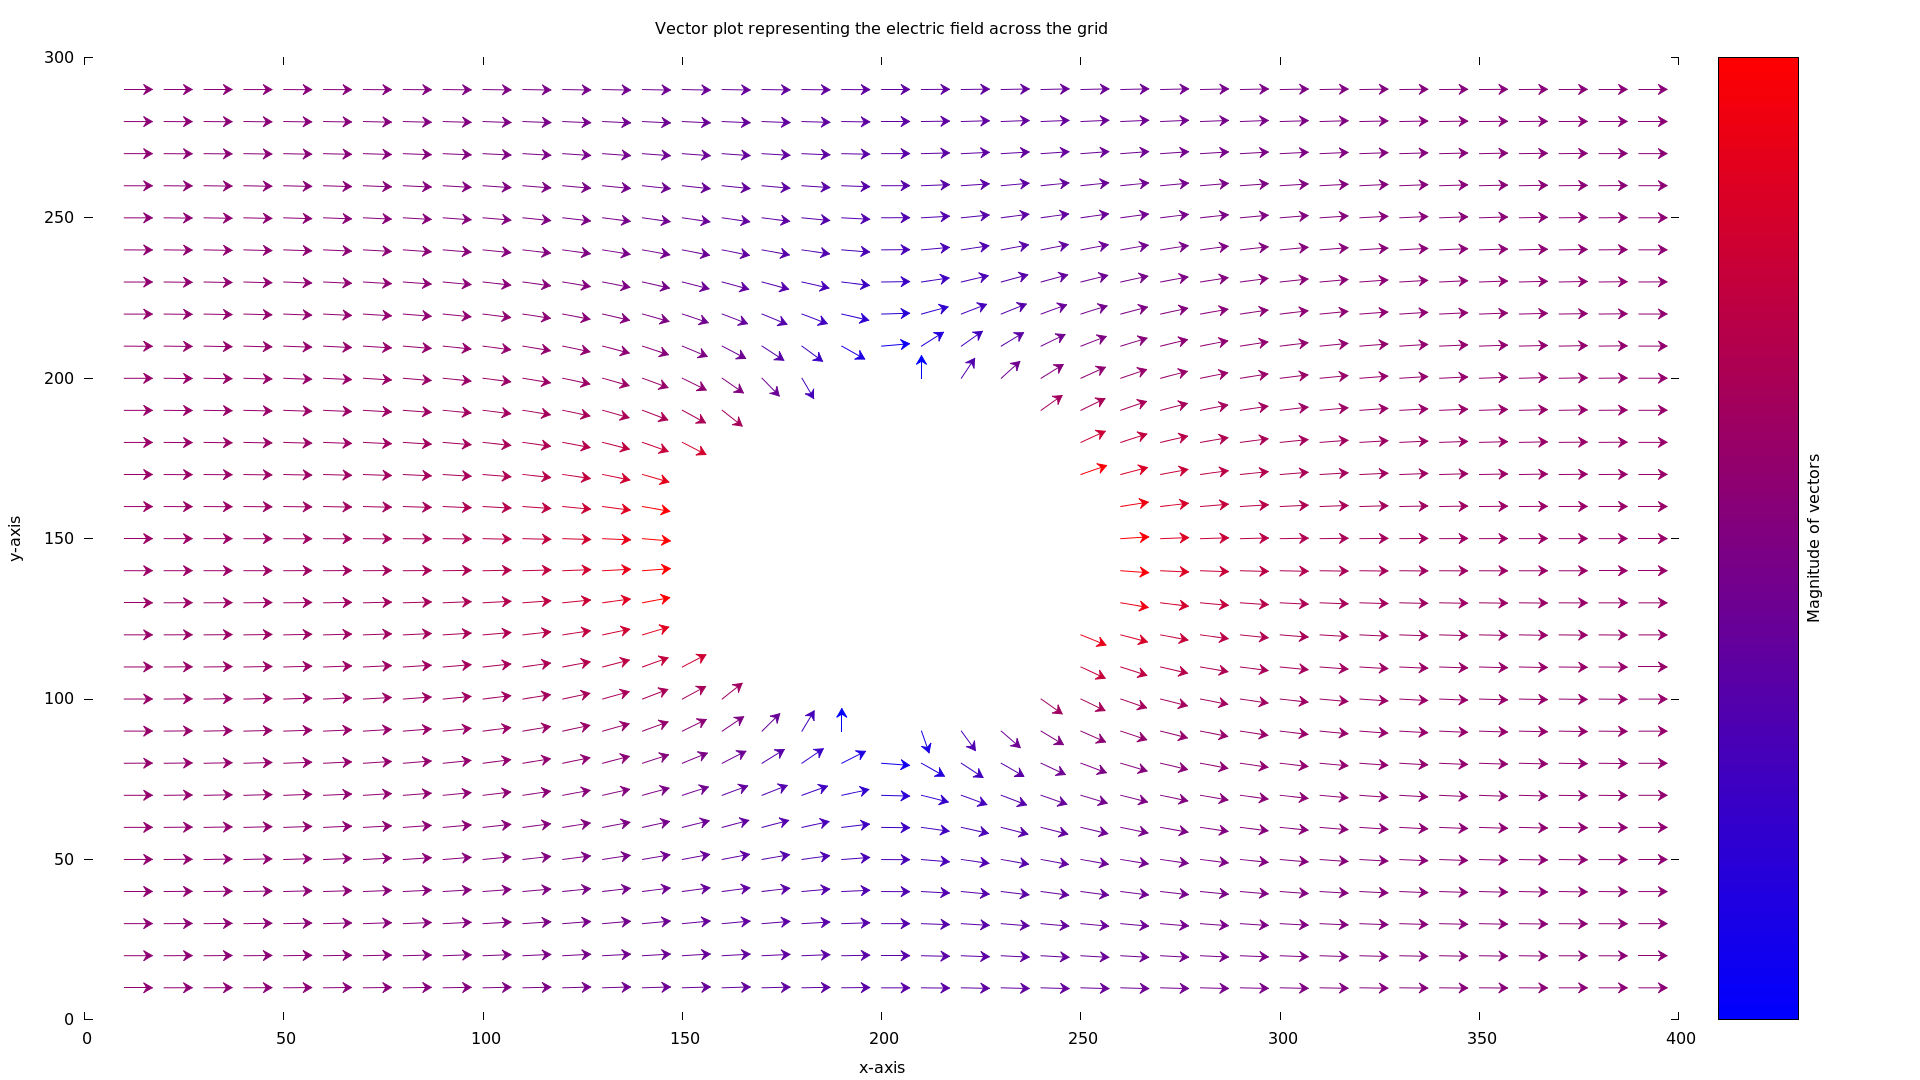
\includegraphics[width=0.95\textwidth, trim = 0mm 0mm 0mm 0mm, clip]{example_vector_field_plot.png}} % trim options: left bottom right top, change to appropriate values if some other image is used and it has too much whitespace around it.
    \caption{A plot representing the electric field calculated for System A, shown as a vector plot with the colour of the vectors indicating the magnitude of the vector: red means large, blue means small.}
    \label{fig:vectorfieldplot}
\end{figure}
 
An equipotential plot is also produced. This uses the same data file as the heatmap-styled plot. The equipotential lines are drawn by the contour function in gnuplot. An example of an equipotential line plot overlaid on a vector field can be seen in figure \ref{fig:vectors_and_contours}.

\begin{figure}[h!]
    \centering
    \setlength\fboxsep{0pt}
    \setlength\fboxrule{0.5pt}
    \fbox{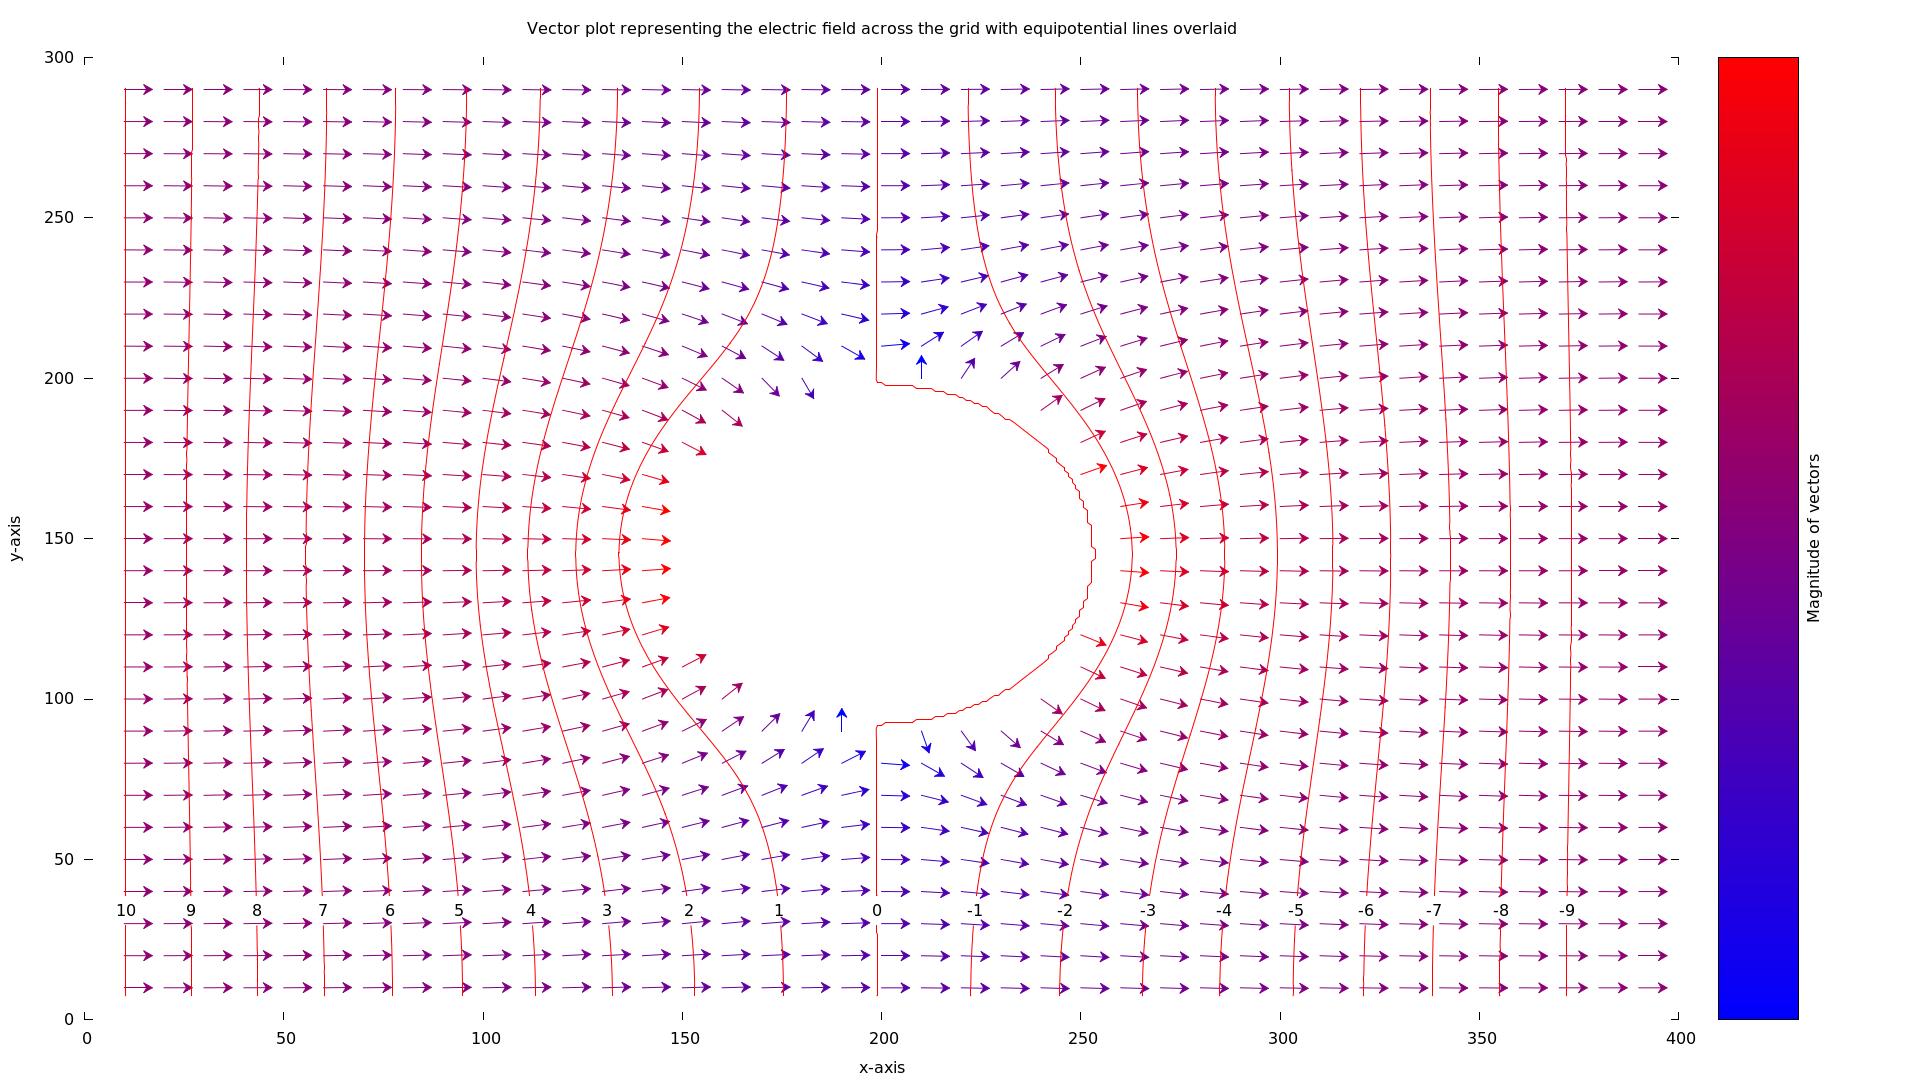
\includegraphics[width=0.95\textwidth, trim = 0mm 0mm 0mm 0mm, clip]{example_vectors_and_contours.png}} % trim options: left bottom right top, change to appropriate values if some other image is used and it has too much whitespace around it.
    \caption{A plot displaying the electric field represented as vectors with equipotential lines overlaid on top of them.}
    \label{fig:vectors_and_contours}
\end{figure}

All of the plotting in the program is done internally via C++ functions which call gnuplot to be run. The source code can be found in the appendix \ref{code:plot.cpp}.

\end{document}

\subsection{Results}

%start of section
\section{Conclusion}

\subsection{Further Work}

%include BibTex bibliography
\bibliography{report}

%start of appendix
\appendix
\section{Appendices}

\end{document} %end of document
